\documentclass[../main.tex]{subfiles}

\begin{document}


\appendix

\chapter{Supplemental figures}
\label{cha:supplfig}

\begin{figure}[ht]
  \centering
  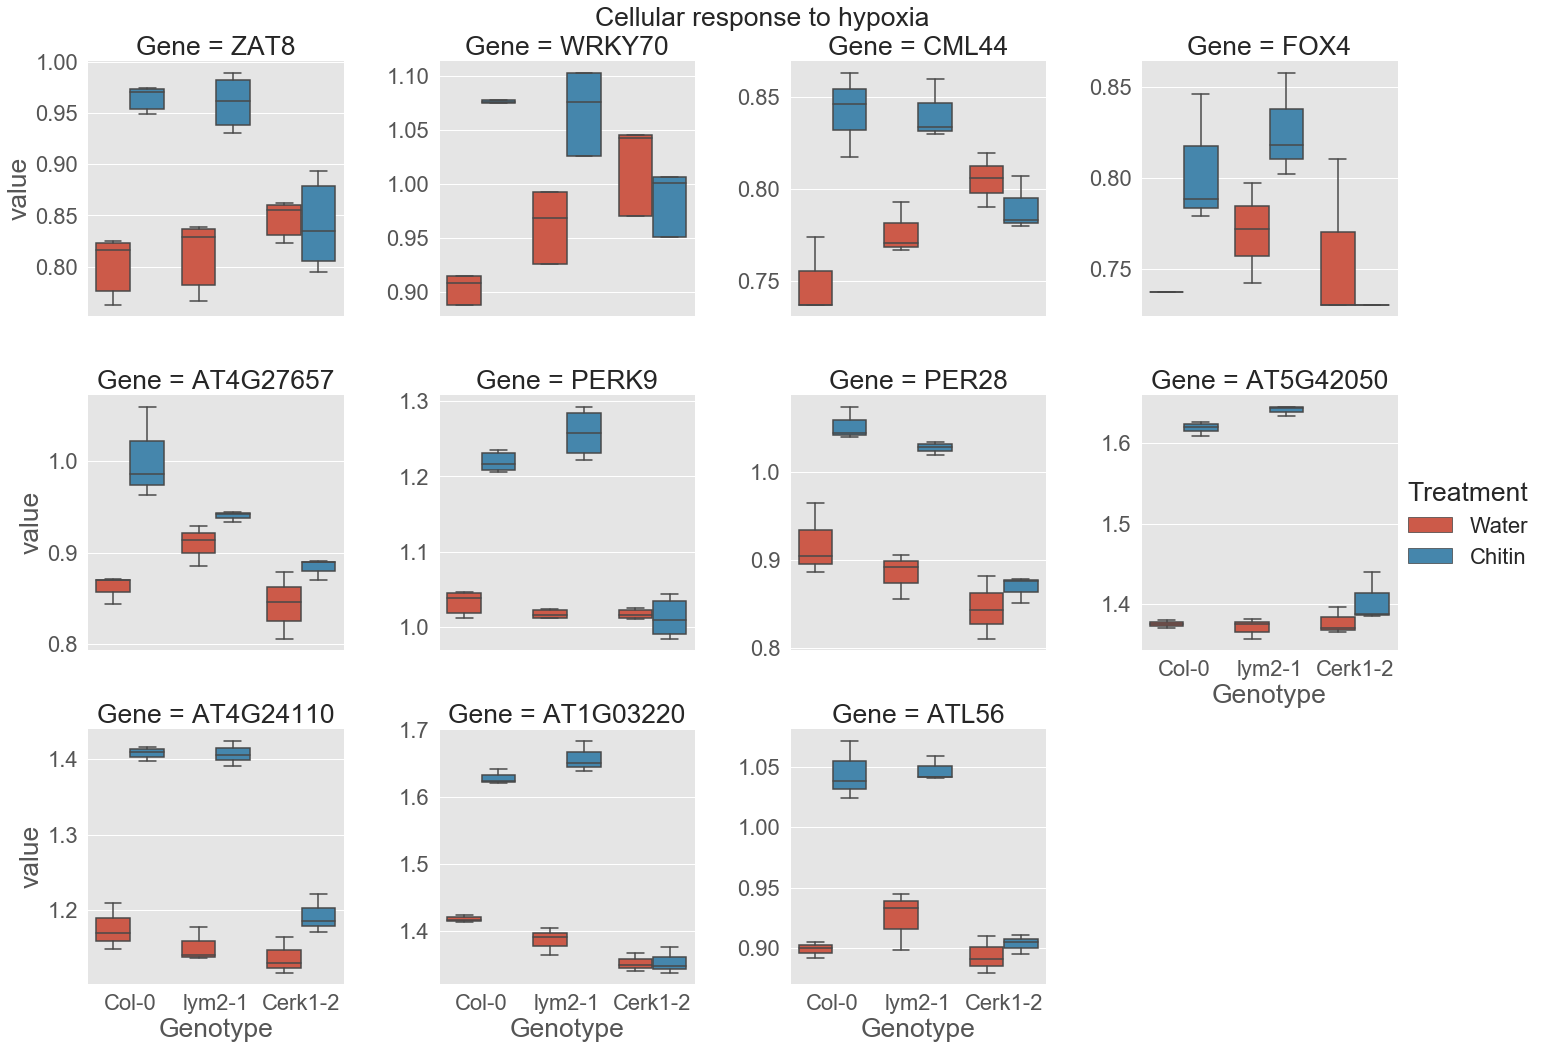
\includegraphics[width=\textwidth, height=\textheight, keepaspectratio]{figures/cellular response to hypoxia.png}
  \caption{\label{fig:resphypoxia} Response to hypoxia}
\end{figure}




\begin{figure}[ht]
  \centering
  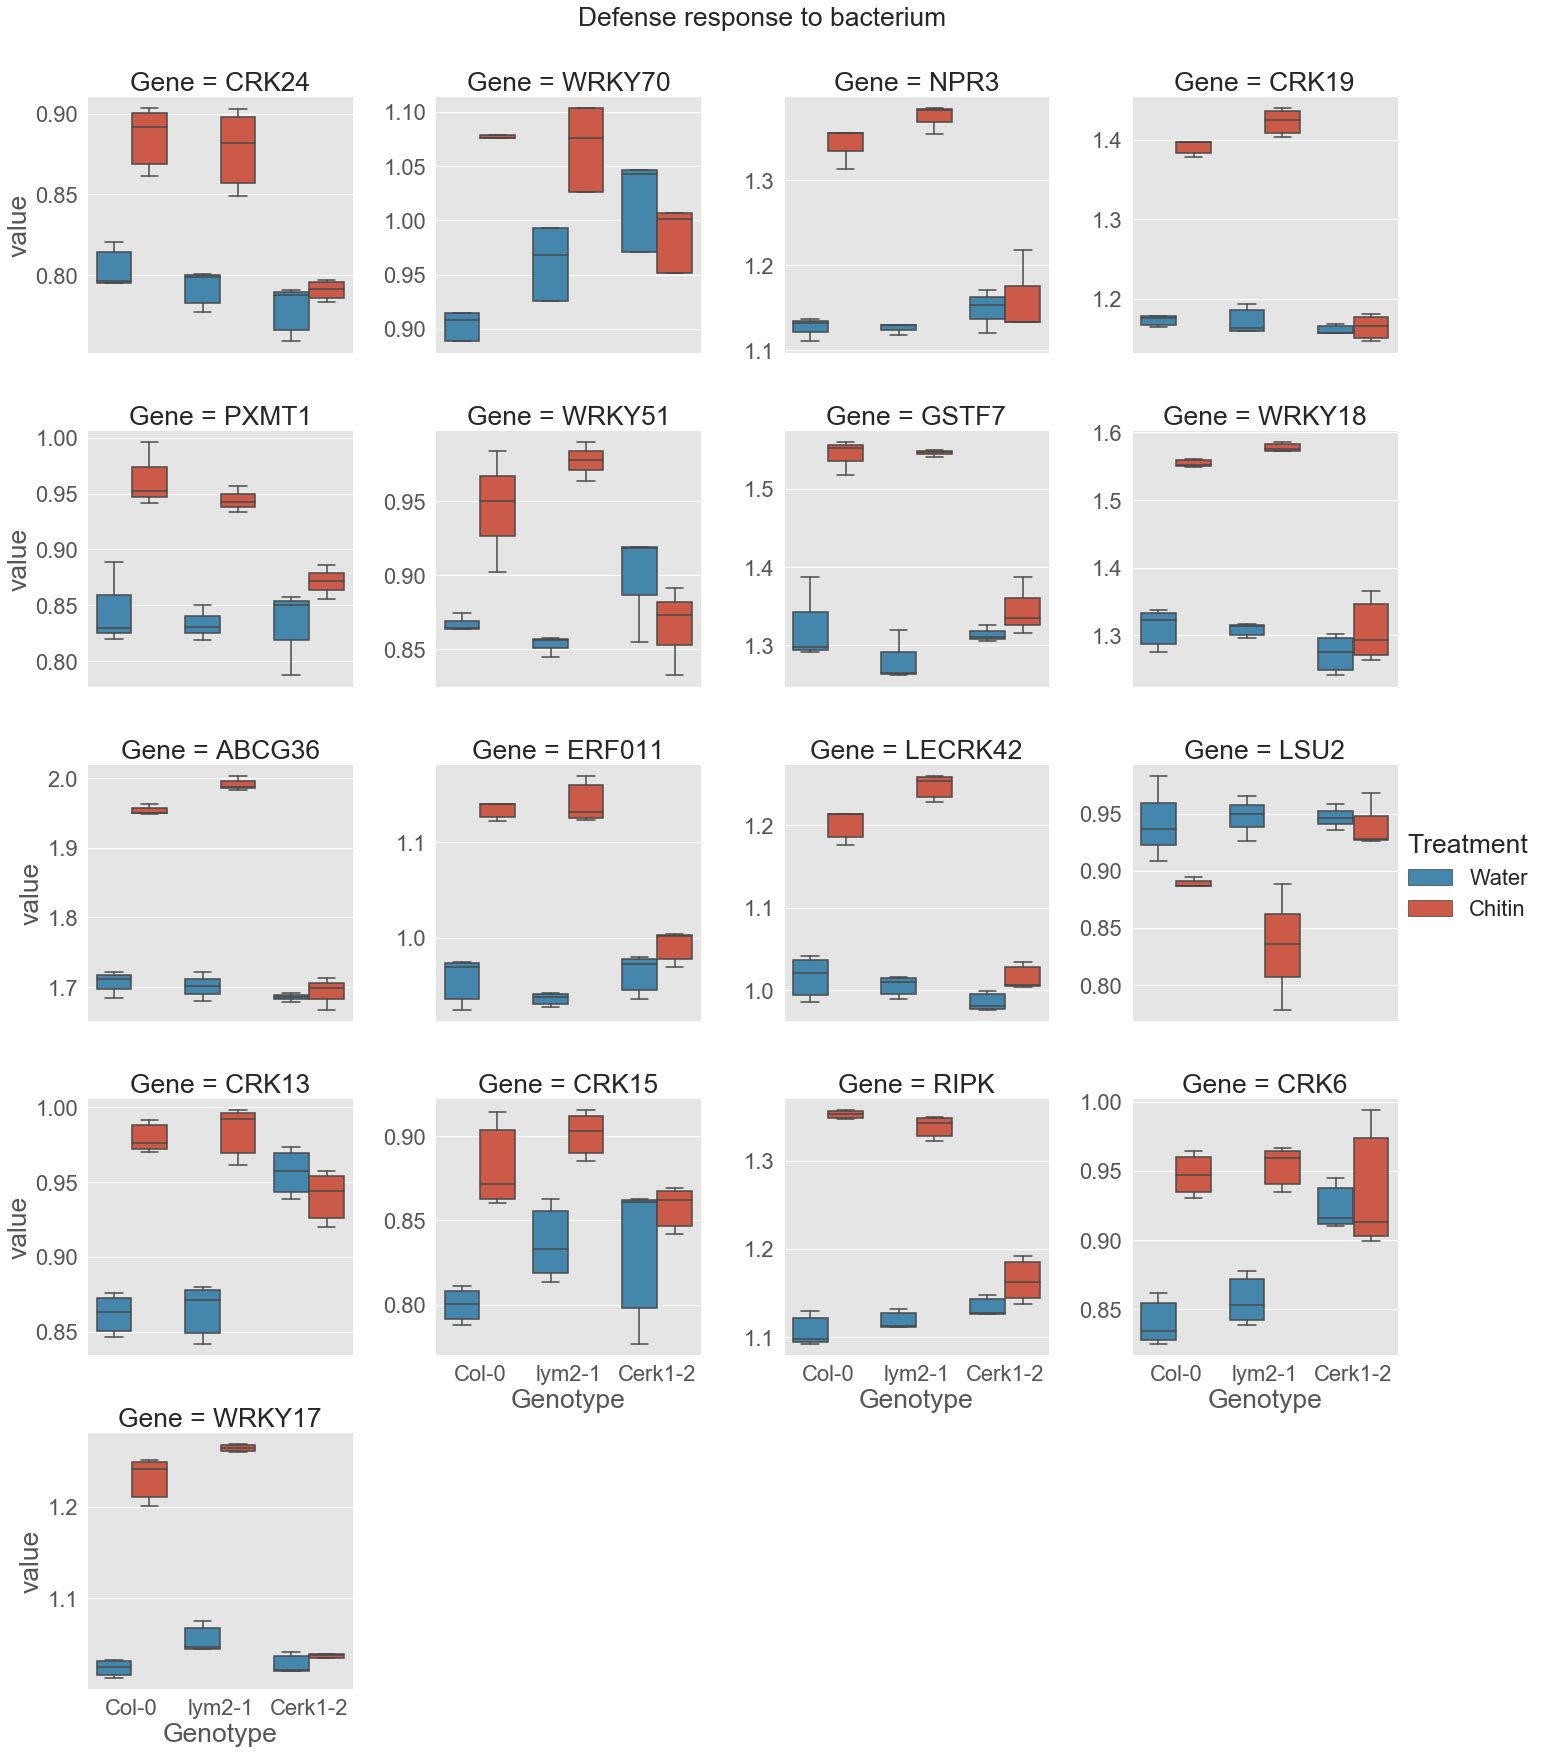
\includegraphics[width=\textwidth,height=\textheight, keepaspectratio]{figures/defense response to bacterium.png}
  \caption{\label{fig:defbacterium} defence response to bacterium}
\end{figure}


\begin{figure}[ht]
  \centering
  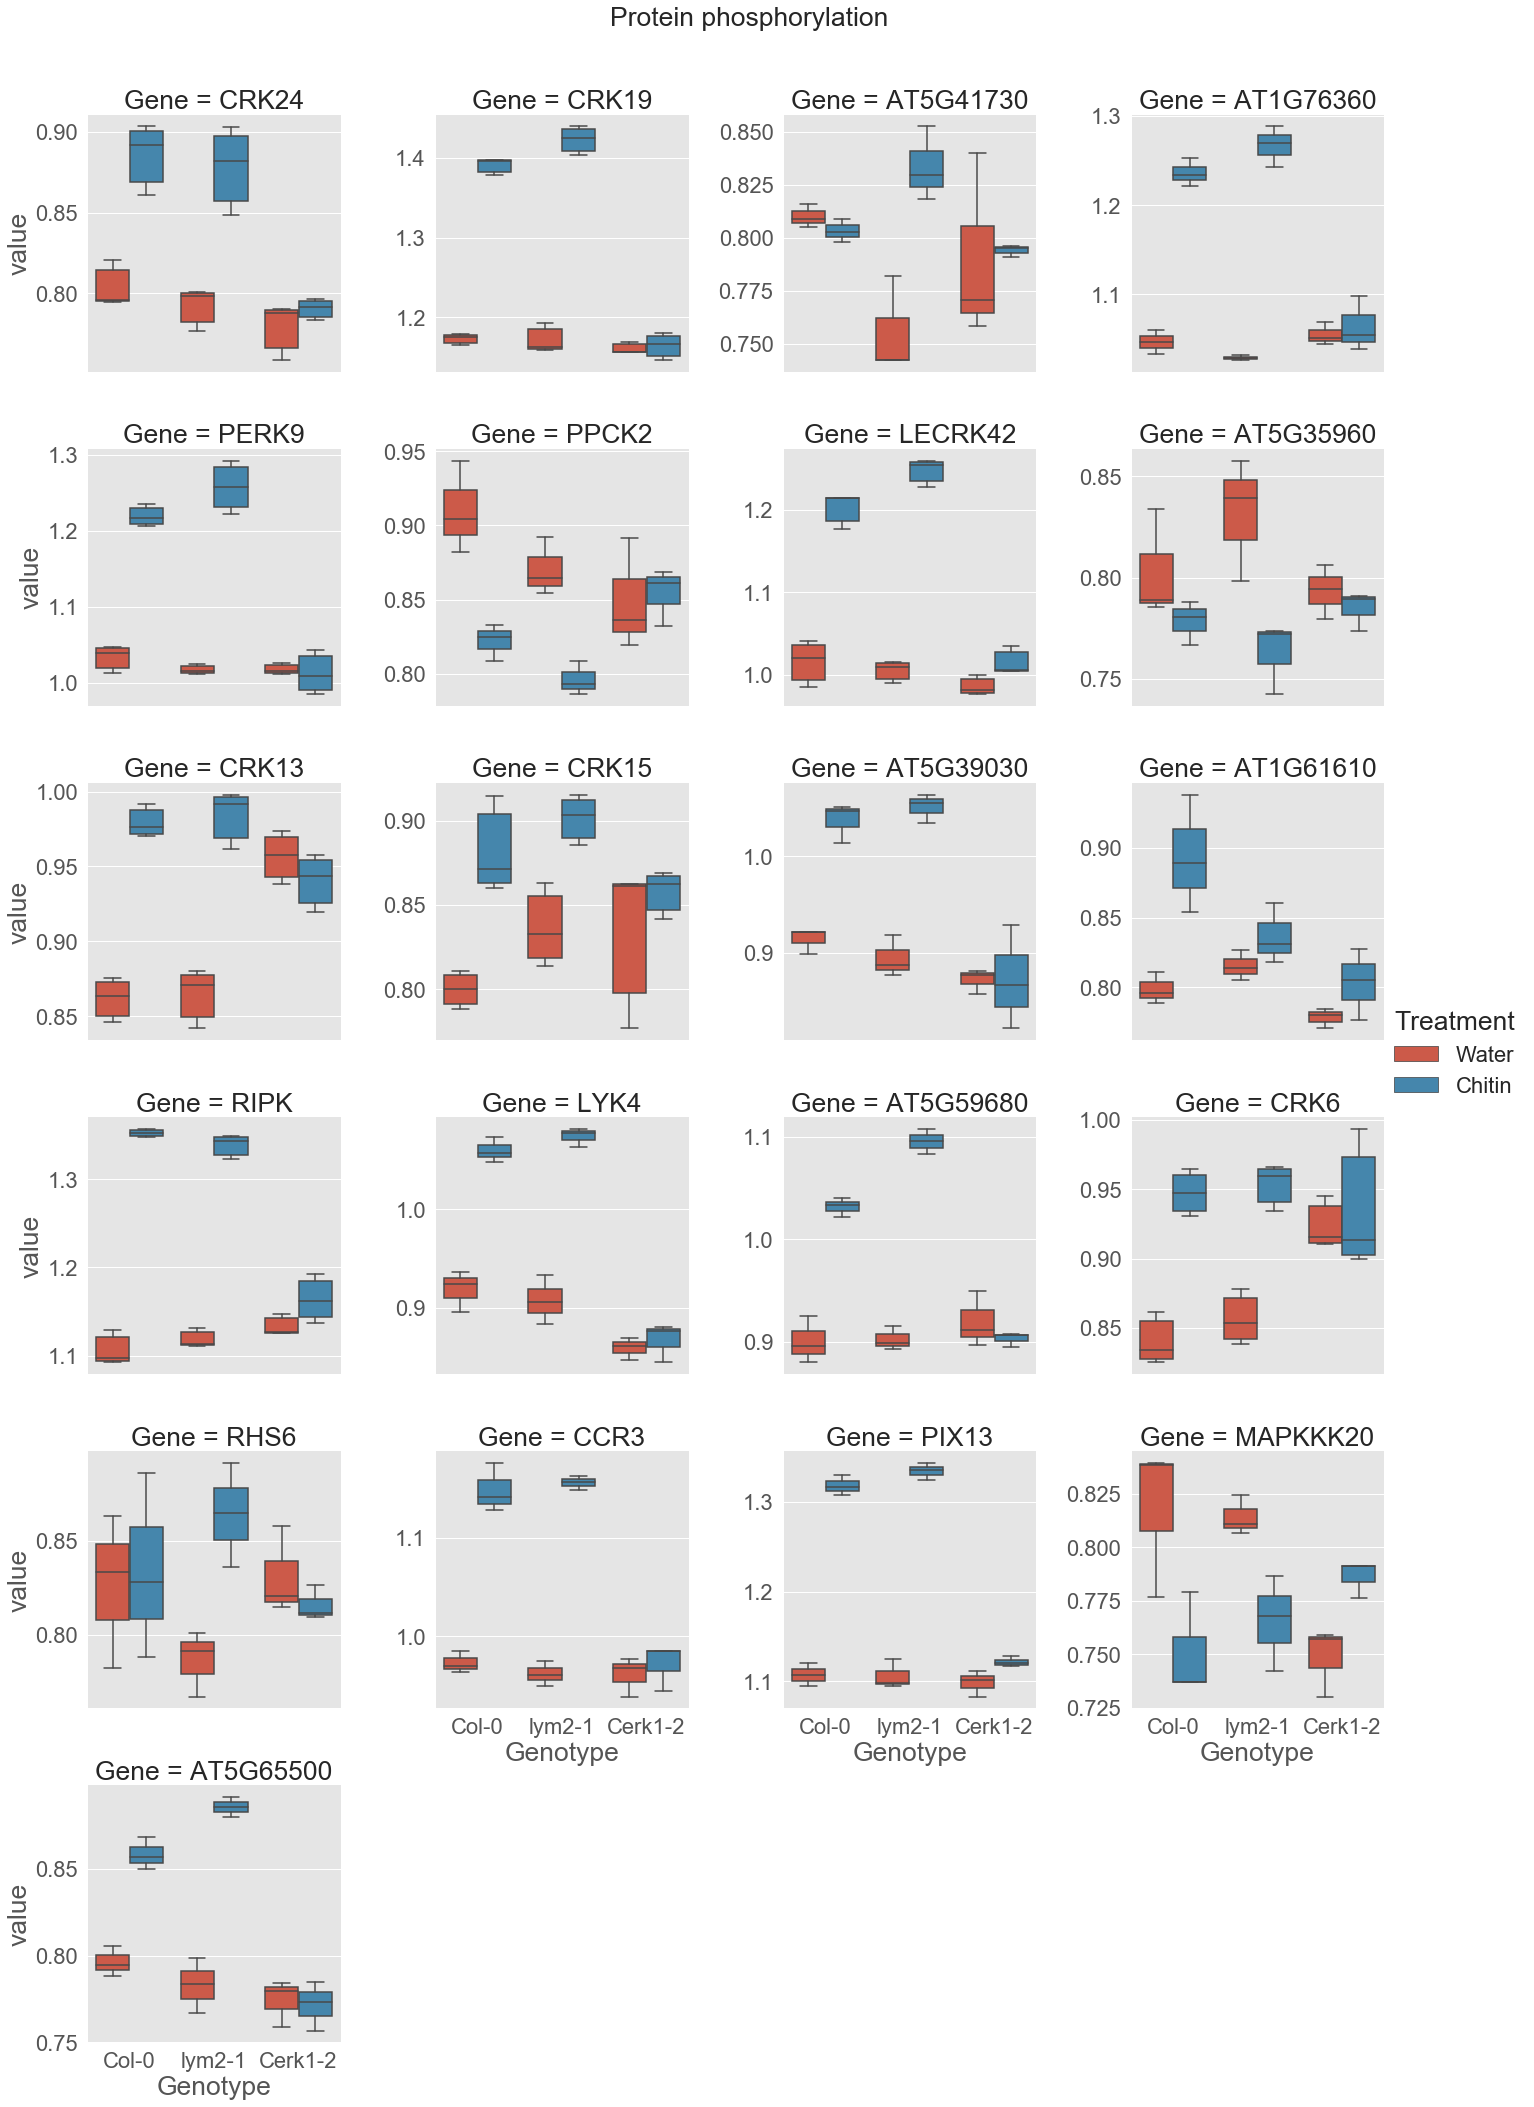
\includegraphics[width=\textwidth, height=\textheight, keepaspectratio]{figures/protein phosphorylation.png}
  \caption{\label{fig:phosphorylation} Protein phosphorylation}
\end{figure}

\end{document}


\chapter{Supplemental tables}
\label{cha:suppltbl}

\section{Col0 GO terms and associated genes}
\label{sec:col0GOgenes}

\begin{longtable}{llp{5cm}ll}
  \caption{Col0 at 05hr significant GO terms, and their associated genes.
  Direction of differential regulation is also shown}\\
  \textbf{AT Code}  & \textbf{Alt. name}  & \textbf{Description} & \textbf{GO Term} & \textbf{Regulation}  \\
  \hline
  AT2G21210 & AT2G21210 & SAUR-like auxin-responsive protein family                                                   & response to chitin            & down          \\
  AT3G50310 & MAPKKK20  & MKKK20                                                                                      & protein phosphorylation       & down          \\
  AT1G61610 & AT1G61610 & Serine/threonine-protein kinase                                                             & protein phosphorylation       & up            \\
  AT2G05940 & RIPK      & Serine/threonine-protein kinase RIPK                                                        & protein phosphorylation       & up            \\
  AT4G23140 & CRK6      & cysteine-rich RLK (RECEPTOR-like protein kinase) 6                                          & protein phosphorylation       & up            \\
  AT4G23230 & CRK15     & Cysteine-rich receptor-like protein kinase 15                                               & protein phosphorylation       & up            \\
  AT2G24570 & WRKY17    & WRKY transcription factor 17                                                                & defense response to bacterium & up            \\
  AT4G23230 & CRK15     & Cysteine-rich receptor-like protein kinase 15                                               & defense response to bacterium & up            \\
  AT3G56400 & WRKY70    & Probable WRKY transcription factor 70                                                       & defense response to bacterium & up            \\
  AT2G05940 & RIPK      & Serine/threonine-protein kinase RIPK                                                        & defense response to bacterium & up            \\
  AT4G23140 & CRK6      & cysteine-rich RLK (RECEPTOR-like protein kinase) 6                                          & defense response to bacterium & up            \\
  AT2G24570 & WRKY17    & WRKY transcription factor 17                                                                & response to chitin            & up            \\
  AT3G56400 & WRKY70    & Probable WRKY transcription factor 70                                                       & response to chitin            & up            \\
  AT3G50060 & MYB77     & Transcription factor MYB77                                                                  & response to chitin            & up            \\
  AT3G46080 & ZAT8      & Zinc finger protein ZAT8                                                                    & response to chitin            & up            \\
  AT5G46910 & AT5G46910 & Transcription factor jumonji (Jmj) family protein  & response to chitin            & up            \\
  AT1G64380 & ERF061    & Ethylene-responsive transcription factor ERF061                                             & response to chitin            & up            \\
  AT1G21550 & CML44     & Probable calcium-binding protein CML44                                                      & cellular response to hypoxia  & up            \\
  AT3G46080 & ZAT8      & Zinc finger protein ZAT8                                                                    & cellular response to hypoxia  & up            \\
  AT3G56400 & WRKY70    & Probable WRKY transcription factor 70                                                       & cellular response to hypoxia  & up            \\
  AT4G27657 & AT4G27657 & At4g27657                                                                                   & cellular response to hypoxia  & up            \\
  AT1G26410 & FOX4      & Berberine bridge enzyme-like 6                                                              & cellular response to hypoxia  & up            \\
  AT2G18670 & ATL56     & RING-H2 finger protein ATL56                                                                & cellular response to hypoxia  & up            \\
\end{longtable}




\section{lym2-1 GO terms and associated genes}
\label{sec:lym2GOgenes}


\begin{longtable}{llp{5cm}ll}
  \caption{lym2-1 at 05hr significant GO terms, and their associated genes.
  Direction of differential regulation is also shown}\\
  \textbf{AT Code}  & \textbf{Alt. name}  & \textbf{Description} & \textbf{GO Term} & \textbf{Regulation}  \\
  \hline
  AT3G04530 & PPCK2     & Phosphoenolpyruvate carboxylase kinase 2                             & protein phosphorylation       & down  \\
  AT5G35960 & AT5G35960 & Protein kinase family protein                                        & protein phosphorylation       & down  \\
  AT5G24660 & LSU2      & Protein RESPONSE TO LOW SULFUR 2                                     & defense response to bacterium & down  \\
  AT5G42050 & AT5G42050 & DCD (Development and Cell Death) domain protein                      & cellular response to hypoxia  & up    \\
  AT3G03670 & PER28     & Peroxidase 28                                                        & cellular response to hypoxia  & up    \\
  AT1G68690 & PERK9     & Proline-rich receptor-like protein kinase PERK9                      & cellular response to hypoxia  & up    \\
  AT1G03220 & AT1G03220 & Eukaryotic aspartyl protease family protein                          & cellular response to hypoxia  & up    \\
  AT4G24110 & AT4G24110 & NADP-specific glutamate dehydrogenase                                & cellular response to hypoxia  & up    \\
  AT5G59450 & SCL11     & Scarecrow-like protein 11                                            & response to chitin            & up    \\
  AT3G16530 & AT3G16530 & Lectin-like protein At3g16530                                        & response to chitin            & up    \\
  AT1G08930 & ERD6      & ERD6                                                                 & response to chitin            & up    \\
  AT4G31800 & WRKY18    & WRKY like transcription factor                                       & response to chitin            & up    \\
  AT5G47220 & ERF2      & ERF2                                                                 & response to chitin            & up    \\
  AT3G50260 & ERF011    & Ethylene-responsive transcription factor ERF011                      & response to chitin            & up    \\
  AT4G23210 & CRK13     & Cysteine-rich receptor-like protein kinase 13                        & defense response to bacterium & up    \\
  AT3G53810 & LECRK42   & L-type lectin-domain containing receptor kinase IV.2                 & defense response to bacterium & up    \\
  AT3G50260 & ERF011    & Ethylene-responsive transcription factor ERF011                      & defense response to bacterium & up    \\
  AT1G59870 & ABCG36    & ABC transporter G family member 36                                   & defense response to bacterium & up    \\
  AT4G23270 & CRK19     & cysteine-rich RLK (RECEPTOR-like protein kinase) 19                  & defense response to bacterium & up    \\
  AT1G66700 & PXMT1     & Paraxanthine methyltransferase 1                                     & defense response to bacterium & up    \\
  AT4G23320 & CRK24     & cysteine-rich RLK (RECEPTOR-like protein kinase) 24                  & defense response to bacterium & up    \\
  AT5G45110 & NPR3      & NPR3                                                                 & defense response to bacterium & up    \\
  AT5G64810 & WRKY51    & Probable WRKY transcription factor 51                                & defense response to bacterium & up    \\
  AT4G31800 & WRKY18    & WRKY like transcription factor                                       & defense response to bacterium & up    \\
  AT1G02920 & GSTF7     & Glutathione S-transferase F7                                         & defense response to bacterium & up    \\
  AT5G41730 & AT5G41730 & Protein kinase family protein                                        & protein phosphorylation       & up    \\
  AT1G76360 & AT1G76360 & At1g76360                                                            & protein phosphorylation       & up    \\
  AT2G17220 & PIX13     & Probable serine/threonine-protein kinase PIX13                       & protein phosphorylation       & up    \\
  AT4G23210 & CRK13     & Cysteine-rich receptor-like protein kinase 13                        & protein phosphorylation       & up    \\
  AT5G65500 & AT5G65500 & U-box domain-containing protein kinase family protein                & protein phosphorylation       & up    \\
  AT3G53810 & LECRK42   & L-type lectin-domain containing receptor kinase IV.2                 & protein phosphorylation       & up    \\
  AT5G39030 & AT5G39030 & Probable receptor-like protein kinase At5g39030                      & protein phosphorylation       & up    \\
  AT4G23270 & CRK19     & cysteine-rich RLK (RECEPTOR-like protein kinase) 19                  & protein phosphorylation       & up    \\
  AT2G23770 & LYK4      & LysM domain receptor-like kinase 4                                   & protein phosphorylation       & up    \\
  AT5G59680 & AT5G59680 & Probable LRR receptor-like serine/threonine-protein kinase At5g59680 & protein phosphorylation       & up    \\
  AT4G23320 & CRK24     & cysteine-rich RLK (RECEPTOR-like protein kinase) 24                  & protein phosphorylation       & up    \\
  AT1G68690 & PERK9     & Proline-rich receptor-like protein kinase PERK9                      & protein phosphorylation       & up    \\
  AT1G51880 & RHS6      & root hair specific 6                                                 & protein phosphorylation       & up    \\
  AT3G55950 & CCR3      & Putative serine/threonine-protein kinase-like protein CCR3           & protein phosphorylation       & up           
\end{longtable}                                                                                                                                                             








%%% Local Variables:
%%% mode: latex
%%% TeX-master: "../main"
%%% End:
